\documentclass[12pt, letterpaper]{report}
\usepackage{graphicx}
\usepackage{hyperref}
\usepackage{amssymb}
\usepackage{amsmath}
\usepackage{float}
\usepackage{mathtools}
\usepackage{enumitem}
\usepackage[margin=1in]{geometry}
\usepackage[figurename=Figura]{caption}
\title{E2 Segundo examen argumentativo}
\author{Juan Pablo Guerrero Escudero A01706810}
\date{29 abril, 2024}
\begin{document}
\maketitle
\subsection*{Problema 1}
\begin{enumerate}
\item Determina el volumen de aire que encierra esta superficie usando integrales dobles. 
Para determinar el volumen de aire que encierra ésta superficie usando integrales dobles, primero es necesario plantear la región de integración, 
que puede ser de tipo 1 o de tipo 2. En éste caso, al observar el plano xy de la figura, observamos que no existe discontinuidad 
entre ambas curvas, es decir, el área de integración siempre empieza en una curva y termina en otra. Por lo tanto, planteamos la 
región de integración como Tipo 1, es decir, x se mueve entre constantes, y "y" se ajusta a los valores de $x$ 
por medio de dos funciones. Si observamos el siguiente diagrama de la región de integración, se observa que tenemos una circunferencia como traza, con ecuación $x^2 + y^2 = 1$, es decir, 
una circunferencia con radio 1. Por lo tanto, x se mueve de -1 a 1, y $y$ se mueve de acuerdo a la ecuación de la traza, y si despejamos para $y$, $y = \pm \sqrt{1-x^2}$, que 
corresponde a la parte positiva y negativa de la circunferencia. Por lo tanto, 
\begin{figure}[H]
    \centering
    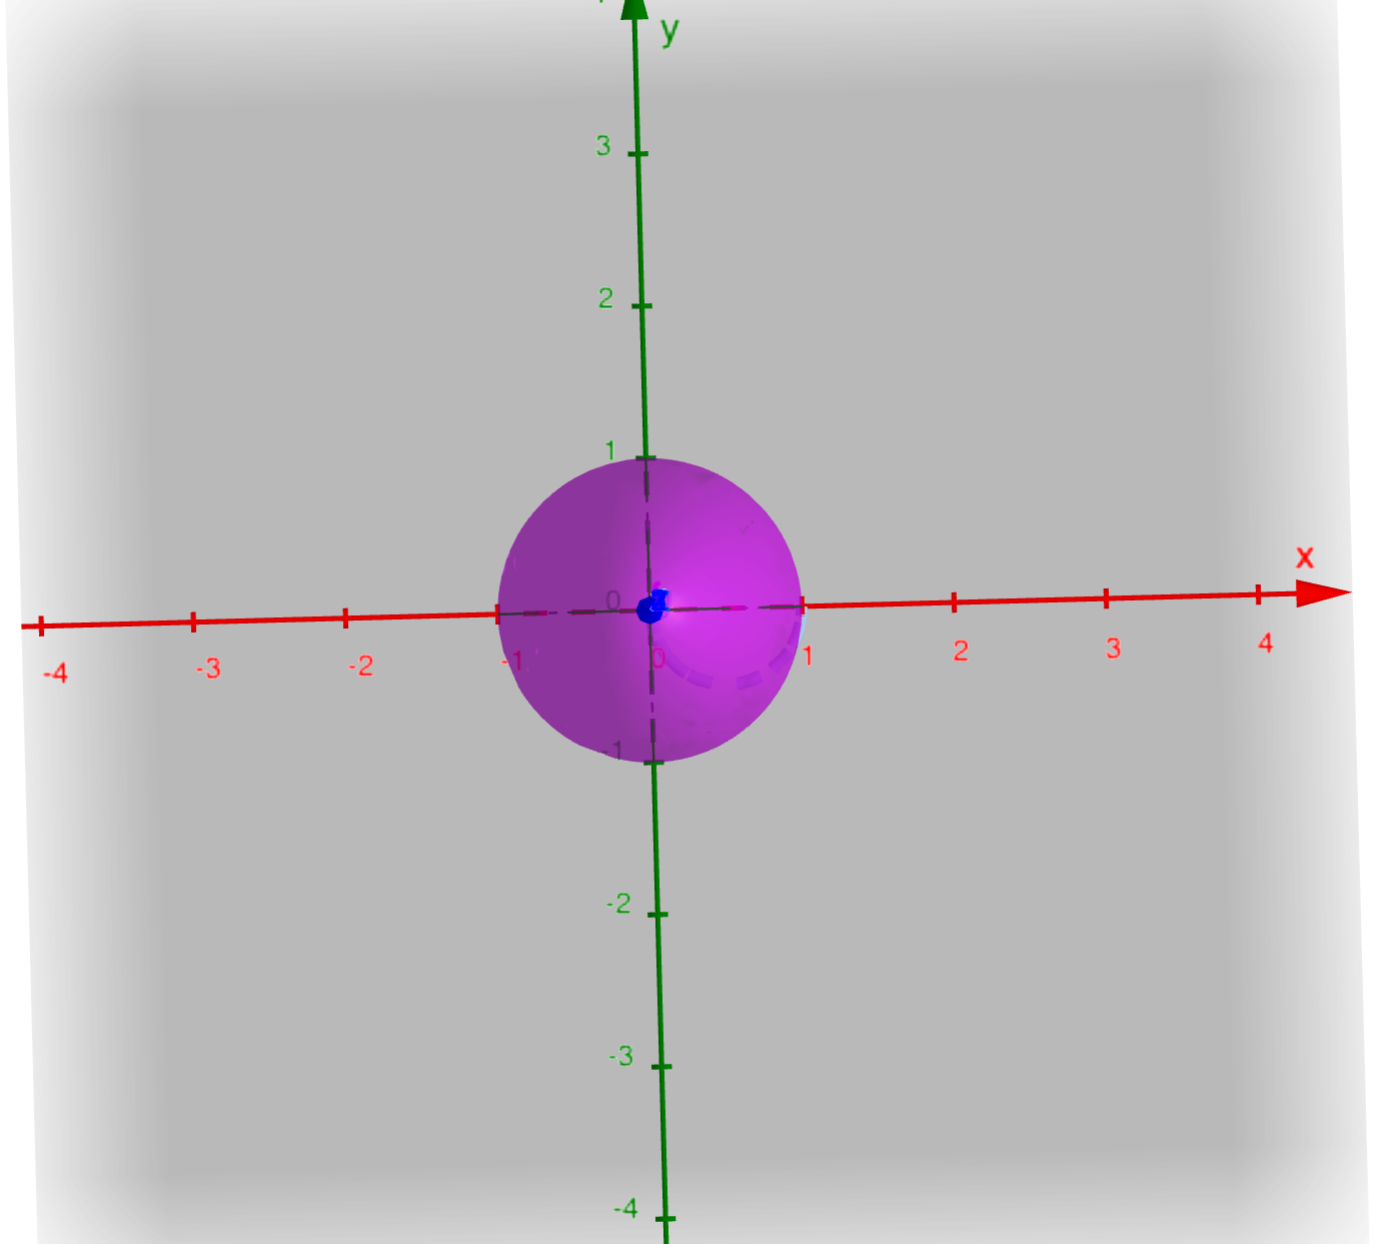
\includegraphics[height = 5cm]{Diagrama 1.png}
    \caption{Diagrama de la región de integración del inciso 1}
\end{figure}
\begin{align}
D_I = \{ (x, y) \in \mathbb{R}^2 | -1\leq x \leq 1, -\sqrt{1-x^2} \leq y \leq \sqrt{1-x^2}\} 
\end{align}
Y así, como tenemos una ecuación, podemos resolver en primer lugar para $y$ con el fin de obtener 
una forma de función, y haciendo ésto resulta $y = \pm 3\sqrt{-x^2 -y^2 -1}$. Que nos da la parte 
tanto positiva como negativa de nuestra superficie. Tomamos solo la parte positiva ya que el problema menciona que la 
superficie está por encima del plano $xy$. \\ 

Ahora, podemos plantear la integral doble para obtener el volumen de la estructura, y ya que la región de integración definida 
anteriormente es de tipo 1, $V = \int \int_{D_I} f(x, y)dA$, y sustituyendo cada componente por lo obtenido anteriormente: 
\begin{align}
\int_{-1}^{1} \int_{-\sqrt{1-x^2}}^{\sqrt{1-x^2}} 3\sqrt{-x^2 -y^2 +1}dydx
\end{align} La cual nos da el volumen de la superficie por encima del plano xy. Resolviendo con Wolfram, resulta $V = 2\pi \approx 6.2832 m^3$. Es decir, 
el volumen de la superficie cuádrica es igual a $2\pi m^3$. Lo cual es congruente con lo esperado ya que el valor es positivo, indicando 
un volumen positivo, y además el valor obtenido tiene una magnitud adecuada. 

\item Determinar el volumen del área superficial de la porcion de la superficie dentro del cilindro con ecuación $(x^2 - 1/2)^2 + y^2 = \frac{1}{4}$, y comprobar si 
1L de pintura es suficiente, que rinde para $5 m^2$. 
En primer lugar, para determinar el área superficial, tenemos que hacer una integral doble ya que estamos trabajando en $R^3$. Lo primero, es plantear la región de integración. Como vemos en la siguiente figura del 
cilindro en el plano xy, observamos que la región de integración siempre es continua, es decir, si un eje se mueve entre constantes, el otro siempre se ajusta y sus puntos 
terminan sobre una misma curva. Así, planteamos la región de integración de Tipo 1, donde $x$ se mueve entre constantes, y $y$ se ajusta a $x$ por medio de dos funciones. \\ 
\begin{figure}[H]
    \centering
    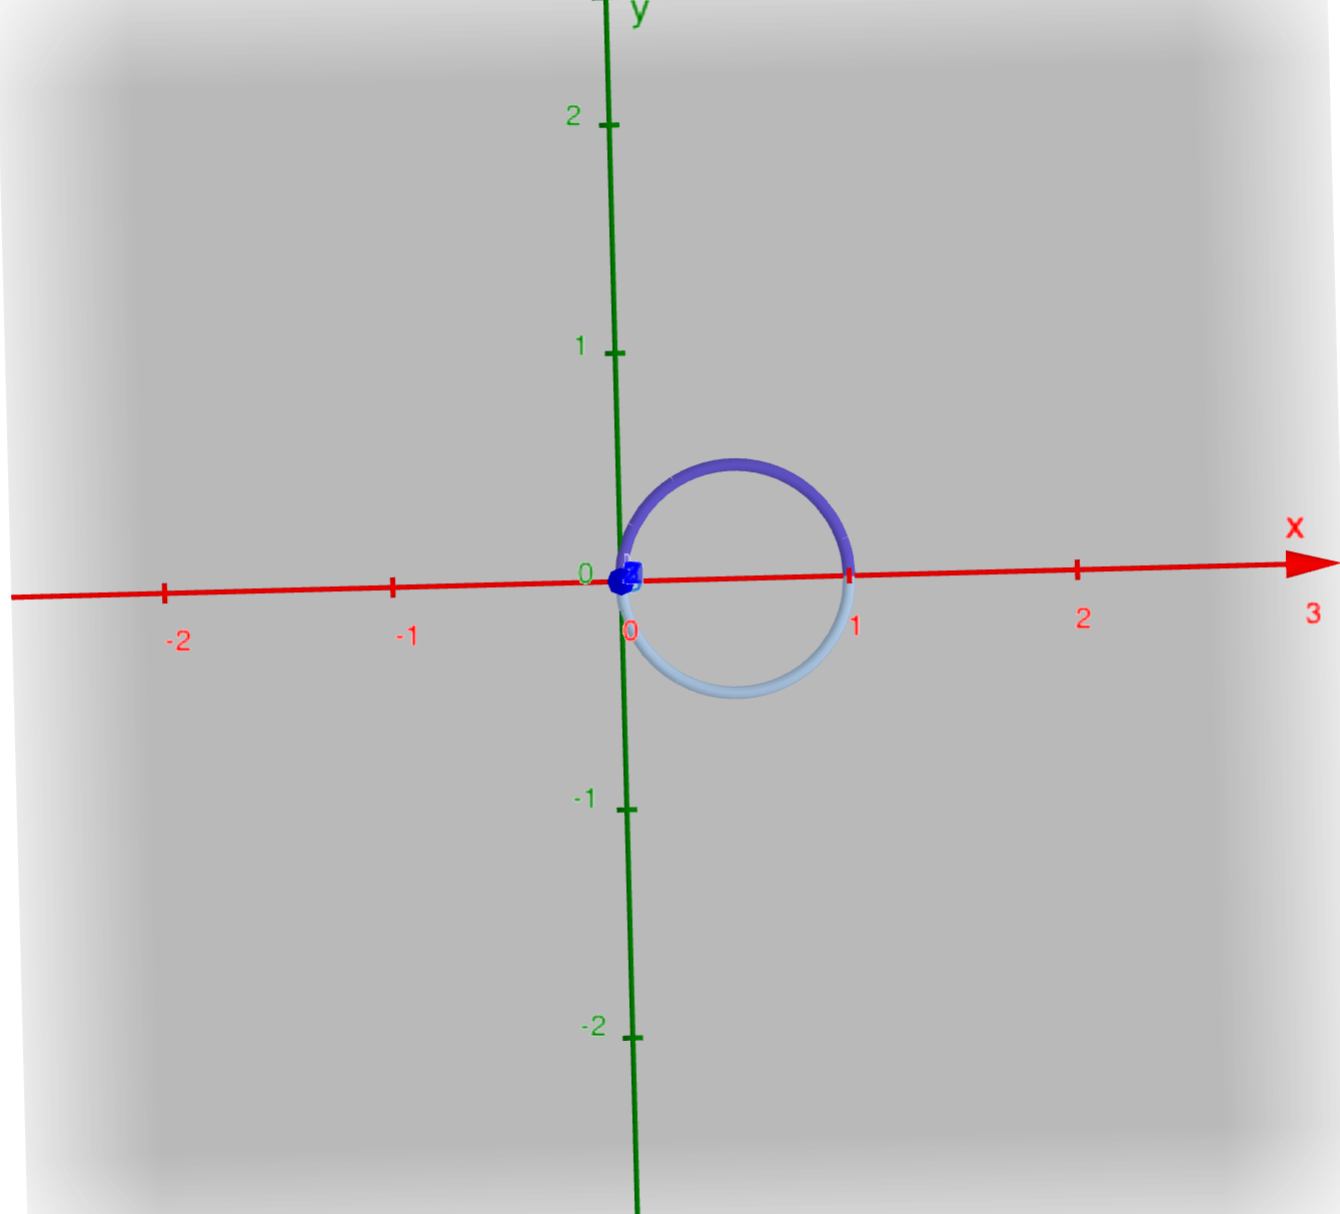
\includegraphics[height = 5cm]{Diagrama 2.png}
    \caption{Diagrama de la región de integración del área superficial}
\end{figure}

En primer lugar, se observa que $x$ se mueve de $0$ a $1$, y para encontrar la ecuación que describe al movimiento en $y$, 
podemos resolver la función dada del cilindro de región de integración para $y$, la cuál resulta $y = \pm \sqrt{\frac{1}{4} - (x-\frac{1}{2})^2}$. Que 
corresponde a la parte negativa y positiva del cilindro. Ahora, podemos plantear la región de integración con notación de conjuntos: 
\begin{align}
D_I = \{ (x, y) \in \mathbb{R}^2 | 0 \leq x \leq 1,-\sqrt{\frac{1}{4} - (x-\frac{1}{2})^2} \leq y \leq \sqrt{\frac{1}{4} - (x-\frac{1}{2})^2} \} 
\end{align}
Teniendo la región de integración, nos dice los límites de integración, y por lo tanto podemos plantear la integral doble de la misma manera que en el inciso 1, usando la fórmula de 
área superficial $A_s = \int\int_D \sqrt{(D_xf)^2 + (D_yf)^2 + 1}dA$. Al obtener las derivadas parciales respecto a $x$ y $y$ de la función $f(x, y) = 3\sqrt{-x^2 -y^2 -1}$ ya que solo 
nos interesa la parte por encima del plano xy, calculado con Matlab resulta que $D_xf = -\frac{3x}{\sqrt{-x^2-y^2+1}}$, $D_yf = -\frac{3y}{\sqrt{-x^2-y^2+1}}$. Y por lo tanto, sustituyendo lo anterior 
en la fórmula de área superficial, con una región de integración Tipo 1, resulta:
\begin{align}
\int_{0}^{1} \int_{-\sqrt{\frac{1}{4} - (x-\frac{1}{2})^2}}^{\sqrt{\frac{1}{4} - (x-\frac{1}{2})^2}} \sqrt{(-\frac{3x}{\sqrt{-x^2-y^2+1}})^2+(-\frac{3y}{\sqrt{-x^2-y^2+1}})^2 +1}dydx
\end{align}
y resolviendo con Wolfram la ecuación anterior, resulta que $A_s = 2.41021$, lo cuál nos dice que el área superficial de la figura dentro del cilindro es de $2.41021 m^2$. Por lo tanto, 
sí será suficiente el litro de pintura, ya que éste rinde para $5m^2$, y como tenemos de área superficial $2.41021m^2$, es suficiente. 
\end{enumerate}

\subsection*{Situación 2}
\subsubsection{Esfera}
\begin{enumerate}
\item Valor de la altura: 
Para calcular el valor de la altura de la esfera con ecuación $x^2 + y^2 + z^2 = 100$, primero podemos 
reescribir la ecuación en términos de $x$ y $y$ para obtener la forma de una función. Haciendo ésto, resulta $z = f(x, y) = \pm \sqrt{100 -x^2 - y^2}$. Que 
corresponde a la parte por encima y por debajo del eje $x$ de la esfera. Entonces, para calcular la altura en el punto $(5, 3)$ sustituimos éstos valores en la función positiva, 
la cual nos da un valor de $z$ que corresponde a la altura. Entonces, $f(5, 3) = \sqrt{66} \approx 8.124m$. 
\item Razón de cambio de la altura desde el punto $(5, 3)$ hacia el punto $(0, 0)$. Para obtener la razón de cambio desde el punto $P = (5, 3)$ en dirección al origen, 
utilizamos el concepto de derivada direccional, que nos dicen el cambio que tiene una función en cierta dirección, dada por un vector unitario $u = <a, b>$. Para esto, primero obtenemos el vector 
que nos dice la dirección de la derivada direccional, la cuál es $v = (-5, -3)$ ya que el punto se dirige hacia el origen. Después, como éste vector no es unitario, es decir, 
no tiene magnitud 1, calculamos su norma y de ahí dividimos cada componente de $v$ para obtener el vector unitario $u$. $||u|| = \sqrt((-5)^2 + (-3)^2) = \sqrt(34)$, y por lo tanto $v = (-\frac{5}{\sqrt{34}}, -\frac{3}{\sqrt{34}})$. 
Ahora, la fórmula de la derivada direccional es $D_uf(x_0, y_0) = D_xf(x_0, y_0)a + D_yf(x_0, y_0)b$, donde $a, b$ son las componentes del 
vector unitario, y cada uno se multiplica por la derivada parcial en $x$ o en $y$. Calculando las derivadas parciales de la función con Matlab, resulta $D_xf = -\frac{x}{\sqrt{-x^2 - y^2 + 100}}$, y $D_yf = -\frac{y}{\sqrt(-x^2 - y^2 + 100)}$. \\ 

Calculando lo anterior, obtenemos que $D_uf(5, 3) = 0.7177$, es decir, la función crece $0.7177m$ por cada metro avanzado en dirección del vector unitario. 
\item Si la dirección de máximo crecimiento es la dirección indicada en el punto anterior, es decir, desde 
el punto dado y en dirección al punto máximo $(0, 0)$: La dirección de máximo crecimiento es aquella en la que apunta el vector gradiente, y por lo tanto para saberla en la función anterior calculamos el vector gradiente 
y evaluamos en el punto $(5, 3)$ para obtener la dirección de máximo crecimiento. El vector gradiente es $\nabla f = (-\frac{x}{\sqrt{-x^2 - y^2 + 100}}, -\frac{y}{\sqrt(-x^2 - y^2 + 100)})$, y evaluando $\nabla f(5, -3) = (0.6155, 0.3693)$, que es la 
dirección de máximo crecimiento. Además, si calculamos la norma de éste vector, $||\nabla f(5, 3)|| = 0.7177$, y como éste corresponde 
con el punto anterior, podemos decir que la dirección de máximo crecimiento es la dada en el inciso anteiror. 
\item Puede existir algún punto donde la dirección de máximo crecimiento sea $\theta = 2\pi / 3$. Para hacer esto, recordamos que la máxima tasa de cambio en un punto está dada por el vector gradiente $||\nabla f(x_0, y_0)||$. Aquí, no existe 
ningún punto en el que la dirección de máximo cambio sea $\theta = 2\pi / 3$, ya que la máxima razón de cambio está dada en el punto $(5, 3)$ mencionado anteriormente, la cuál es 0.7177, y al la magnitud del vector gradiente con dirección en 
$\theta = 2\pi / 3$, obtenemos que la razón de cambio en ese punto, en esa dirección es igual a $-0.0121$, lo cuál es menor que el gradiente, y por lo tanto al ser éste el punto de máximo cambio, 
no puede haber un punto en donde $\theta = 2\pi / 3$ corresponda a la dirección de máximo cambio. 
\end{enumerate}
\end{document}
